\documentclass[11pt]{article}
\usepackage{graphicx}
\usepackage[spanish]{babel}
\usepackage{multirow}
\usepackage{cite}
\usepackage{textpos}
\usepackage{hyperref}
\usepackage{comment}


\begin{document}
\begin{titlepage}

\begin{textblock}{3}(0,11.5)
   \begin{tabular}{ccc}
      Puebla, Pue. & \phantom{MMMMMMMMMMMMMMMMM} & Mayo de 2024\phantom{MMMMMM}
   \end{tabular}
\end{textblock}

\centering
\phantom{M}

\vspace{-20mm}
{
\includegraphics[width=4cm]{buap} \par}
\vspace{5mm}
{\bfseries\huge Benem\'{e}rita Universidad Aut\'{o}noma de Puebla \par}
\vspace{10mm}
{\Large Facultad de Ciencias Qu\'{i}micas\par}
{\Large Centro de Qu\'{i}mica-Instituto de Ciencias \par}
\vspace{5mm}
{\Large Posgrado en Ciencias Qu\'{i}micas\par}
\vspace{15mm}
{\textbf{``La dimensi\'{o}n fractal de masa como medida caracterizadora\\de la estructura de las prote\'{i}nas''} \par}
\vspace{15mm}
{\large Protocolo de Tesis de Maestr\'{i}a\par}
\vspace{5mm}
{\Large Lic. en Qu\'{i}mica \par}
{\Large Edgar Garc\'{i}a Ju\'{a}rez \par}
\vspace{20mm}


\begin{tabular}{p{0.45\textwidth}cp{0.45\textwidth}}
  \cline{1-1} \cline{3-3} \\
  \centering Director de tesis \\ Dr. J. Manuel Solano Altamirano & & \centering Co-Directora de tesis\\ Dra. Viridiana Vargas Castro 
\end{tabular} 

\end{titlepage}

%-----------------------------------------------------------------------------%
% Cover Page
%-----------------------------------------------------------------------------% 
\clearpage

\section{Introducci\'{o}n}

Los cristal\'{o}grafos han observado durante mucho tiempo que las prote\'{i}nas son pol\'{i}meros muy compactos. Sin embargo, la estructura nativa que se captura en un cristal es, aunque representativa, solo  una de las muchas que una prote\'{i}na puede adoptar durante el curso de su funci\'{o}n en la c\'{e}lula viva. La noci\'{o}n de que las prote\'{i}nas son simplemente objetos tridimensionales extremadamente compactos puede ser demasiado simple. De hecho, se ha señalado desde hace tiempo la posibilidad de que las prote\'{i}nas puedan estar mejor caracterizadas por la geometr\'{i}a fractal en lugar de objetos tridimensionales compactos \cite{Enright2005, Dewey1997}. Adicionalmente, el problema de cuantificar las diferencia entre dos estructuras de una misma prote\'{i}na no es trivial y contin\'{u}a evolucionando \cite{Kufareva2012}. Una de las medidas  cuantitativas m\'{a}s comunes para 
determinar la similitud entre dos conjuntos de coordenadas at\'{o}micas 
es la Desviaci\'{o}n Cuadr\'{a}tica Media 
(RMSD, por sus siglas en ingl\'{e}s). El uso del RMSD es crucial en campos como la bioqu\'{i}mica 
y la qu\'{i}mica computacional porque permite comparar modelos generados por 
simulaciones o experimentos para verificar su similitud con estructuras 
conocidas, como prote\'{i}nas o complejos moleculares. 
No obstante, el RMSD puede ser engañoso cuando se trata de diferencias
 locales significativas. Por ejemplo, al analizar dos estructuras que difieren solo 
 en un segmento pequeño, deben tener un RMSD global, similar a pesar de que existan partes
 altamente movibles, lo que dificulta el an\'{a}lisis. Por esta raz\'{o}n, encontrar
  m\'{e}todos alternativos o enfoques complementarios para comparar estructuras 
  es fundamental. Estas alternativas podr\'{i}an enfocarse en las regiones clave,
   permitiendo a los investigadores ignorar las variaciones menores y 
  centrarse en las partes cr\'{i}ticas de las estructuras \cite{Kufareva2012}.

Dicho lo anterior, la dimensi\'{o}n fractal puede sintetizar toda la informaci\'{o}n que contienen los sistemas prote\'{i}cos. Adem\'{a}s, desde hace varios años, la dimensi\'{o}n fractal de masa se ha utilizado para identificar la distribuci\'{o}n de distintos patrones, \textit{v. gr.}, sistemas magnetoreol\'{o}gicos (piedras, polvos magnetizados o geles envejecidos) \cite{Carrillo2003}. Lo anterior sucede porque cuando se mide la dimensi\'{o}n fractal de masa a diferentes escalas, se puede obtener  informaci\'{o}n acerca de los patrones de agregaci\'{o}n; adem\'{a}s, se ha observado la aparici\'{o}n de c\'{u}mulos  con propiedades multifractales, mostrando un comportamiento lineal.

Regresando a las prote\'{i}nas, autores como Matthew \textit{et al.} \cite{Enright2005} han calculado la dimensi\'{o}n fractal de varias prote\'{i}nas de forma global, sin el an\'{a}lisis de varias etapas de agregaci\'{o}n. Es decir, sin analizar c\'{o}mo cambian los patrones de agregaci\'{o}n cuando se cambia la escala de medici\'{o}n de la dimensi\'{o}n fractal de masa.

El an\'{a}lisis multifractal encontrado por Carrillo \textit{et al.} \cite{Carrillo2003}, aplicado a diferentes tipos de estructuras (no simplemente a geles envejecidos), podr\'{i}a servir para extraer informaci\'{o}n de los patrones de agregaci\'{o}n de otros objetos en diferentes etapas. Se sabe que, en las prote\'{i}nas existe m\'{a}s de una etapa de agregaci\'{o}n o de conformaci\'{o}n, esto plantea la siguiente pregunta; ¿Se podr\'{i}an detectar estos patrones de agregaci\'{o}n en las prote\'{i}nas midiendo la dimensi\'{o}n fractal de masa en este esquema de objetos multifractales? De ser cierto lo anterior, ¿ser\'{i}a esta medida lo suficientemente precisa para distinguir entre dos prote\'{i}nas con secuencias gen\'{e}ticas similares pero estructuralmente diferentes? Para responder a estas interrogantes, es fundamental desarrollar una herramienta computacional que nos permita calcular la dimensi\'{o}n fractal de masa y llevar a cabo pruebas exhaustivas. Es importante resaltar que, de ser cierto lo anterior, se podr\'{i}a abrir la puerta a futuras aplicaciones en enfermedades. No obstante, a\'{u}n no se sabe con certeza si es posible observar la multifractalidad en prote\'{i}nas, por lo que este trabajo se enfocar\'{a} en determinar si se observa.


\section{Antecedentes}

\subsection{Fractal y dimensi\'{o}n fractal}
\label{subsec:subseccion2.1}


Existen objetos que tienen la propiedad de que su geometr\'{i}a tenga una apariencia fragmentada o con una morfolog\'{i}a aparentemente irregular y que no cambia a cualquiera que sea la escala a la que se analice; a estos objetos se les conoce como fractales. Los fractales est\'{a}n presentes en un gran n\'{u}mero de sistemas complejos que van desde agregados microsc\'{o}picos hasta c\'{u}mulos de galaxias, por lo tanto, existen objetos que se pueden describir en t\'{e}rminos de su geometr\'{i}a fractal \cite{Vicsek1992}. 

La autosimilitud o invariancia de escala es la propiedad m\'{a}s importante en la geometr\'{i}a fractal porque puede modelar la complejidad de cualquier objeto. La dimensi\'{o}n fractal \textbf{(D)} es el \'{i}ndice num\'{e}rico que cuantifica esta complejidad, midiendo la tasa de adici\'{o}n de detalles estructurales con una mayor ampliaci\'{o}n. En la literatura cient\'{i}fica puede encontrase una gran variedad de m\'{e}todos para determinar la dimensi\'{o}n fractal, algunos de ellos son la dimensi\'{o}n fractal Hausdorff-Besicovitch y la dimensi\'{o}n fractal Minkowski.

\subsection{Multifractalidad en geles}
\label{subsec:subseccion2.2}

En \'{e}sta secci\'{o}n, expondremos brevemente el
trabajo que nos inspir\'{o} a proponer este proyecto, 
originalmente utilizado en el \'{a}rea de f\'{i}sica de materiales 
y particularmente en sistemas magnetorreol\'{o}gicos. 

La multifractalidad es una propiedad de ciertos sistemas
 complejos donde la estructura exhibe autosimilitud a m\'{u}ltiples 
 escalas \cite{Posadas2001}. En otras palabras, la distribuci\'{o}n de ciertas 
 caracter\'{i}sticas o propiedades del sistema no es uniforme,
  sino que var\'{i}a de manera heterog\'{e}nea en diferentes 
  escalas espaciales o temporales. Esto significa que diferentes
   partes del sistema pueden exhibir diferentes grados de autosimilitud 
   fractal, lo que resulta en una multifractalidad.

En el caso espec\'{i}fico del sistemas estudiado por  
Carrillo \textit{et al.}\cite{Carrillo2003}, como las dispersiones
 magnetorreol\'{o}gicas y otros conglomerados formados 
 por procesos de agregaci\'{o}n, la multifractalidad se 
 manifiesta en la variaci\'{o}n de la dimensi\'{o}n fractal 
 a lo largo de diferentes etapas del proceso de formaci\'{o}n 
 de estructuras. Esta variaci\'{o}n indica que la autosimilitud
  fractal no es constante, sino que cambia a medida que se 
  desarrollan diferentes interacciones y se forman conglomerados 
  de distintas generaciones. Como se observa en el gr\'{a}fico \ref{fig:Carrillo2003},
   existen tres porciones claramente distinguibles, asociadas a las tres etapas 
   de agregaci\'{o}n mencionadas anteriormente. Cada porci\'{o}n tiene un comportamiento lineal y ha sido ajustada por una l\'{i}nea recta usando el m\'{e}todo de m\'{i}nimos cuadrados. N\'{o}tese la estrecha similitud entre ambas curvas, mostrando porciones rectas que revelan procesos de agregaci\'{o}n claramente similares que generan el patr\'{o}n jer\'{a}rquico \cite{Carrillo2003}.


\begin{figure}[h!]
\vspace{1cm}
\centering
{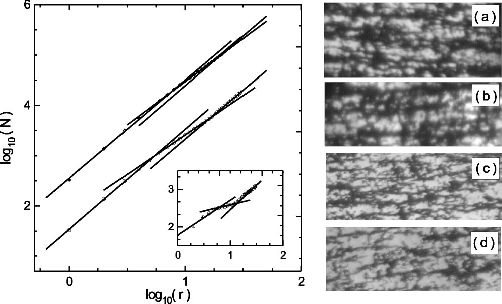
\includegraphics[width=7cm]{Carrillo2006} \par}
\caption{ $\log_{10}N$ vs $\log_{10}r$ para estructuras formadas en un sistema magnetorreológico, para dos fracciones volumétricas de partículas $(\phi)$, los valores de $r$ se expresan en términos del tamaño medio de las partículas $(\sigma)$. Inserción: $\log_{10}(N_i - N_{i-1})$ vs $\log_{10} r_i$. Micrografías de la estructura de conglomerados. Imagen tomada de Carrillo \textit{et al} \cite{Carrillo2003}.}
\label{fig:Carrillo2003}
\end{figure}
 
\clearpage  
\subsection{Determinaci\'{o}n de la dimensi\'{o}n fractal}
\label{subsec:subseccion2.3}


La determinaci\'{o}n de la dimensi\'{o}n fractal de estructuras en crecimiento normalmente resulta de la aplicaci\'{o}n directa de las definiciones para D, sin embargo, esto es ineficaz. 
Es necesario medir o calcular cantidades que se puede demostrar que est\'{a}n relacionadas con la dimensi\'{o}n fractal de los objetos.
 Existen  tres tipos de enfoques principales para la determinaci\'{o}n de estas cantidades: (i) el experimental, (ii) el te\'{o}rico y (iii) el inform\'{a}tico \cite{Vicsek1992}. 
 El enfoque inform\'{a}tico se obtienen digitalizando im\'{a}genes o por procedimientos num\'{e}ricos. Los datos generados num\'{e}ricamente suelen producirse mediante variaciones del m\'{e}todo de Monte Carlo \cite{Mustafa1996}. 
 Para hacer las estimaciones m\'{a}s precisas, generalmente se calcula la dimensi\'{o}n fractal para muchos grupos y se promedia sobre los resultados. 
 Quiz\'{a}s, el m\'{e}todo m\'{a}s simple es usar la definici\'{o}n de  D como se indica en la secci\'{o}n \ref{subsec:subseccion2.1}. 
 Por lo tanto, la dimensi\'{o}n fractal se puede obtener ajustando una l\'{i}nea recta a la parte asint\'{o}tica de los datos, \textit{v. gr.}, usando el m\'{e}todo de m\'{i}nimos cuadrados \cite{Vicsek1992}, v\'{e}ase la figura \ref{fig:Vicsek-Fractal}. 
 En las secciones \ref{subsec:subseccion2.4}, \ref{subsec:subseccion2.5} y \ref{subsec:subseccion2.6} 
 se hablar\'{a} sobre algunos m\'{e}todos para determinar D. 
  
\begin{figure}[h!]
\vspace{1cm}
\centering
{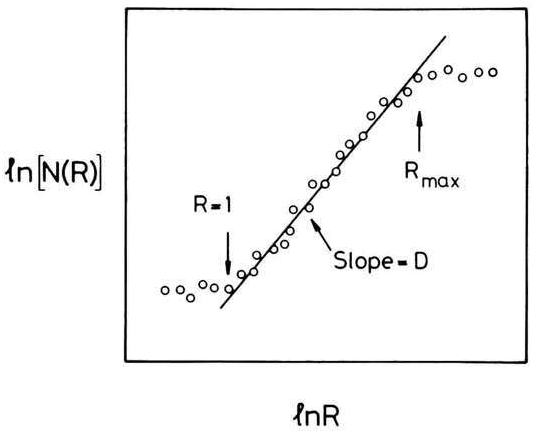
\includegraphics[width=6cm]{Vicsek-Fractal} \par}
\caption{ Gráfico esquem\'{a}tico de $\ln[N(R)]$ vs $\ln (R)$  del número de partículas $N(R)$ que pertenecen a un fractal que se encuentran dentro de una esfera de radio $R$. La dimensión fractal se obtiene ajustando una línea recta a los datos en la región de escala. Imagen tomada del libro \textit{Fractal Growth Phenomena, Tam\'{a}s Vicsek. World Scientific Publishing Company, 1992} \cite{Vicsek1992}.}
\label{fig:Vicsek-Fractal}
\end{figure}
 

\subsection{Relaci\'{o}n entre Masa y radio}
\label{subsec:subseccion2.4}

La relaci\'{o}n masa-radio es \'{u}til para estimar la dimensi\'{o}n de objetos similares a grupos (redes, vasos sangu\'{i}neos, grupos de agregaci\'{o}n). Consiste en seleccionar un punto de origen en el objeto (normalmente el centro de masa) y contar el n\'{u}mero de part\'{i}culas que componen el objeto en un radio del origen. Para un sistema perfectamente homog\'{e}neo la relaci\'{o}n masa-radio es:
\begin{equation}
M(r) \propto r^{2}
\end{equation}

Por ejemplo, el \'{a}rea de un plano bajo discos de tamaño creciente es proporcional al cuadrado del radio del disco de medici\'{o}n. El exponente es la dimensi\'{o}n, pero la masa de un objeto fractal incrustado en dos dimensiones cambia con un exponente fraccionario:

\begin{equation}
M(r) \propto r^{D} 
\end{equation}

Y la dimensi\'{o}n fractal $D_\textit{{masa-radio}}$ se obtiene de:

\begin{equation}
D_\textit{masa radio} = \frac{\log (M(r))}{\log (r)}
\end{equation}

Se calcula como la pendiente de la regresi\'{o}n lineal de $\log(M(r))$ de $\log(r)$ \cite{Mustafa1996}.


\subsection{M\'{e}todo de masa}
\label{subsec:subseccion2.5}


Consiste en selecionar un punto de
 origen en el objeto de estudio (que usualmente es el centro de masa) 
 y contar el n\'{u}mero de part\'{i}culas que componen el objeto en 
 un radio r desde el origen. Para dos dimensiones la relaci\'{o}n 
 entre masa y radio es:

\begin{equation}
\mu(d) = Ad^D
\end{equation}

Donde $\mu(d)$ es el n\'{u}mero de part\'{i}culas en una c\'{i}rculo de di\'{a}metro d, A es un variable y D es la dimensi\'{o}n fractal\cite{Mustafa1996, Nicolás2020}. 

\subsection{Radio de giro}
\label{subsec:subseccion2.6}


Existe una medida que es ocupada por los bioqu\'{i}micos para determinar de forma global, que tan compacta es la estructura de una prote\'{i}na. 
Esta medida es el radio de giro. El radio de giro es la distancia que hay entre cada \'{a}tomo de la mol\'{e}cula a 
su centro de masa. Un valor alto de $R_g$ indica una proteína más extendida, mientras que un radio de giro menor sugiere una proteína más compacta  \cite{Mroczka2012, Vicsek1992}. 
Matemat\'{i}camente se expresa como: 

\begin{equation}
R_g = \sqrt{\frac{\sum_{i} m_{i}r_{i}^{2}}{\sum_{i} m_{i}}}
\end{equation}

Para una partícula rígida, \( m_i \) son los elementos de masa, que est\'{a}n ubicados a una distancia \( r_i \) desde el centro de masa, \(R_g\) es el radio de giro \cite{IUPAC2019}.

   
\subsection{Geometr\'{i}a fractal en prote\'{i}nas}
\label{subsec:subseccion2.6}


Tras establecer la definición de D, exploramos la multifractalidad presente en geles y fluidos magnetorreológicos (ver sección \ref{subsec:subseccion2.2}), y presentamos varios métodos para su determinación. Surge naturalmente la pregunta, ¿La dimensi\'{o}n fractal tiene alguna utilidad?, las respuestas provienen de varios experimentos en los que se ha empleado para cuantificar algunos aspectos de la morfolog\'{i}a proteica. Dado que la estructura de las prote\'{i}nas tiene una forma tan compleja, solo se puede analizar adecuadamente mediante el enfoque de la geometr\'{i}a fractal \cite{Mustafa1996}. 
Es importante recordar que los elementos de la estructura primaria de un prote\'{i}na se le conoce como amino\'{a}cidos. Los elementos de la estructura secundaria de las prote\'{i}nas son las $\alpha$-h\'{e}lices y l\'{a}minas-$\beta$, mientras que la estructura terciaria se relaciona con las disposiciones espaciales de los amino\'{a}cidos en las prote\'{i}nas. La dimensi\'{o}n fractal juega un papel crucial porque se puede utilizar para caracterizar las estructuras terciarias de las prote\'{i}nas y las enzimas \cite{Mustafa1996}. Aunque se pueden construir fractales iterados que son perfectamente autosimilares, la autosimilitud de una cadena de prote\'{i}nas, es similar solo en un sentido estad\'{i}stico, es decir, no siempre se ver\'{a} exactamente como el todo. Otra diferencia entre las macromol\'{e}culas biol\'{o}gicas y los objetos ideales es que una macromol\'{e}cula no es autosimilar desde culquier escala. Hay l\'{i}mites de tamaño superior e inferior m\'{a}s all\'{a} de los cuales una macromol\'{e}cula ya no es un fractal. Por lo que la investigaci\'{o}n fractal sobre enzimas y prote\'{i}nas es actualmente un campo activo \cite{Mustafa1996}. 


\clearpage


\section{Objetivos}
\subsection{Objetivo general}

Determinar si las prote\'{i}nas presentan caracter\'{i}sticas multifractales. De ser as\'{i}, analizar
dicha multifractalidad con el fin de utilizar una o m\'{a}s variantes de la
dimensi\'{o}n fractal como medida(s) caracterizadora(s)
de la estructura y patrones de agregaci\'{o}n de las prote\'{i}nas.


\subsection{Objetivos particulares}

\begin{itemize}

\item Seleccionar un conjunto de prote\'{i}nas de estudio que tengan potencial para aplicaciones posteriores.
Por ejemplo prote\'{i}nas nativas y mutadas, prote\'{i}nas que han mantenido su funci\'{o}n biol\'{o}gica pero que se
han diferenciado estructuralmente, entre otros casos. Se priorizar\'{a}n los casos en que se cuente con informaci\'{o}n
experimental (PDB).

\item Adaptar la determinaci\'{o}n de la dimensi\'{o}n fractal de masa a las prote\'{i}nas, a partir de otros casos como geles o materiales ferromagn\'{e}ticos.

\item Analizar la dimension fractal de masa de un conjunto de prote\'{i}nas, partiendo de la definici\'{o}n de multifractalidad y usando los datos experimentales recabados.

\item Analizar si la multifractalidad de una prote\'{i}na se observa con otras formas de determinar la
dimensi\'{o}n fractal de masa, por ejemplo el radio de giro.

\item Explorar el uso potencial de la dimensi\'{o}n fractal de masa como una herramienta para identificar
o resolver entre prote\'{i}nas gen\'{e}ticamente similares pero con diferencias estructurales notables.

\end{itemize}

\clearpage

\section{Metodolog\'{i}a}

\begin{enumerate}
	
\item Obtenci\'{o}n de las estructuras tridimensionales experimentales de un conjunto de prote\'{i}nas, de alguna base de datos como el \textit{Protein Data Bank} (PDB).

\item C\'{a}lculo de la dimensi\'{o}n fractal de masa: El c\'{a}lculo de la dimensi\'{o}n fractal de masa implica medir c\'{o}mo var\'{i}a el volumen del objeto (en este caso, las prote\'{i}nas) con respecto a la escala a la que se est\'{a} observando. Esto se puede hacer con adaptaciones de los algoritmos conocidos, lo descrito en las secciones \ref{subsec:subseccion2.3} y \ref{subsec:subseccion2.5}.

\item An\'{a}lisis de la complejidad geom\'{e}trica de la prote\'{i}nas: Una vez calculada la dimensi\'{o}n fractal de masa para las prote\'{i}nas, se analizar\'{a} c\'{o}mo var\'{i}a esta dimensi\'{o}n en diferentes escalas. Esto nos permitir\'{i}a caracterizar la complejidad geom\'{e}trica de las prote\'{i}nas a diferentes niveles de detalle.

\end{enumerate}

\clearpage

\section{Cronograma}
\begin{table}[hbp!]
\centering
\footnotesize
\setlength{\tabcolsep}{2.0pt}
\begin{tabular}{||p{0.4\linewidth}|c|c|c|c|c|c|c|c|c|c|c|c||}
\hline
\textbf{Actividad} & \multicolumn{5}{c|}{2023} & \multicolumn{7}{c||}{2024}\\
\hline
& Ago & Sep & Oct & Nov & Dic & Ene & Feb & Mar & Abr & May & Jun & Jul\\
\hline
Materias del primer semestre & X & X & X & X & X & & & & & & &  \\
\hline
LII Winter Meeting on Statistical Physics & & & & & & X & & & & & & \\
\hline
Curso de Qu\'{i}mica Cu\'{a}ntica en \'{a}tomos & & & & & & X & X & X & X & X & X & \\
\hline
Materias del segundo semestre &  &  &  &  &  & X & X & X & X & X & X &\\
\hline
Revisi\'{o}n bibliogr\'{a}fica & X & X & X & X & X & X & X & X & X & X & X & X \\
\hline
Presentaci\'{o}n de protocolo &  &  &  &  &  &  &  &  &  &  & X & \\
\hline
Preparaci\'{o}n de sistemas de estudio  &  &  &  &  &  &  &  &  &  &  &  & X \\
\hline
& \multicolumn{5}{c|}{2024} & \multicolumn{7}{c||}{2025}
\\\hline
& Ago & Sep & Oct & Nov & Dic & Ene & Feb & Mar & Abr & May & Jun & Jul\\
\hline
Asistencia a congreso &  &  &  & X &  &  &  &  &  &  &  &\\
\hline
XXlX Simposio interno FCQ - ICUAP &  &  &  & X &  &  &  &  &  &  &  &\\
\hline
Revisi\'{o}n bibliogr\'{a}fica & X & X & X & X & X & X & X & X & X & X & X &\\
\hline
Redacci\'{o}n de tesis &  &  &  &  &  & X & X & X & X &  &  &\\
\hline
Revisi\'{o}n de tesis &  &  &  &  &  &  &  &  & X & X & X & \\
\hline
Examen &  &  &  &  &  &  &  &  &  &  &  & X\\
\hline
%Actividad &  &  &  &  &  &  &  &  &  &  &  &  \\
\hline
\end{tabular}
\end{table}


\clearpage

\bibliographystyle{plain}
\bibliography{bibliografia}

\end{document}

